%!TEX root = ../thesis.tex

\section{Regular edge labellings}
  Given a layout $\L$ we can thus easily find its adjacency graph and thus for which graph it is a rectangular dual. However, finding a rectangular dual of a triangulation of the $k$-gon $G$ is more involved. Due to the algorithm by He \cite{He1993} it is sufficient to find a \emph{regular edge labeling} on a corner assignment of $G$. In this section we will introduce regular edge labellings.

\mypar{Adjacency graphs of layouts}
  The \emph{ adjacency graph} $\dualgraph{\L}$ of a layout $\L$ each rectangle is represented by a vertex and we connect two vertices by an edge exactly when their rectangles are adjacent. In the \emph{extended adjacency graph} $\extdualgraph{\L}$ we also add $4$ vertices $\pN, \pE, \pS, \pW$ (so-called \emph{poles}) in the outer face, one associated to the north, east, south, west boundary segment of the outer rectangle, respectively. Two vertices are then connected if their rectangles or boundary segments intersect.
  If we take the \emph{extended adjacency graph} of a layout and remove the $4$ vertices corresponding to the outer face we end up with the \emph{adjacency graph} of that layout.
  In this setting a layout $\L$ is a \emph{rectangular dual} of a graph $G$ if we have that $G = \dualgraph{\L}$.


\mypar{Regular edge labellings}
  Regular edge labellings were first introduced by Kant and He \cite{Kant1997} and were also used in \cite{Eppstein2012}. Fusy also studied these structures \cite{Fusy2006,Fusy2009} under the name of \emph{transversal structures}.
  A \emph{regular edge labeling} is a coloring and orientation of the edges of the extended adjacency graph $\extdualgraph{\L}$. This coloring and orientation is given by the following procedure. For every edge $vw$ in $\extdualgraph{\L}$ we consider whether the shared boundary of the rectangles is vertical or horizontal we then color the edge blue or red respectively. In the first case we orient the edge from the leftmost rectangle to the rightmost rectangle and in the second case we orient from bottom to top. We do not color or orient the edges between the poles.

  From the nature of the adjacencies in a rectangular layout we can deduce the following two rules for a regular edge labeling.
  \fxnote{figure, for example from powerpoint}
  \begin{enumerate}
    \item (Interior vertex) In the rotation around every interior vertex we have the following subsequent non-empty sets: Incoming red edges, incoming blue edges, outgoing red edges and outgoing blue edges and only these sets.
    \item (Pole) $\pN$ has only incoming red edges, $\pE$ has only incoming blue edges, $\pS$ has only outgoing red edges and $\pW$ has only outgoing blue edges ,except for the uncolored edges between the poles.
  \end{enumerate}

  In \cite{He1993} He showed that given a regular edge labeling of a corner assignment we can reconstruct a rectangular layout represented by this regular edge labeling.
  A regular edge labeling  of $\ext G$ corresponds to an equivalence class of rectangular layouts $\L$ that are a rectangular dual of $G$.
  \fxnote*{Do we use this anywhere? If so we should proof it.}{A \rel has no monochromatic directed cycles because such a cycle would for example correspond to a  group of adjacent rectangles that have  no leftmost or topmost rectangle.}

  \begin{lemma}
    \label{lm:rel:noMonoColoredTriangles}
    A regular edge labeling has no monochromatic triangles even when ignoring orientation
  \end{lemma}

  \begin{proof}
    Suppose we have a monochromatic triangle. Without loss of generality we suppose that the color of this triangle is blue. Then at least one of the vertices has an incoming blue edge followed directly by an outgoing blue edge or an outgoing blue edge followed directly by an incoming blue edge in its rotation. Thus this vertex has either an empty set of outgoing or incoming red edges, violating the interior vertex requirement of a REL.
  \end{proof}

  \mypar{$\mathbf{st}$-planar graphs}
    In this thesis we repeatedly use regular edge labellings, so it is a good idea to investigate their structure.
    Kant and He \cite{Kant1997} show that a regular edge labeling is closely linked to a pair of $st$-planar graphs. We show this in Theorem \ref{th:rel:stPlanarGraphs} below.

    An $st$-planar graph is an oriented planar graph with one source (in-degree 0) $s$ and one sink (out-degree 0) $t$. Both $s$ and $t$ lie on the outer face. Moreover, such an $st$-planar graph has no directed cycles.

    \begin{thrm}
      \label{th:rel:stPlanarGraphs}
      The blue edges of $G\sm{\pN,\pS}$ form an $st$-planar graph with $s= \pW$ and $t=\pE$. Moreover the red edges of $G\sm{\pW,\pE}$ form an $st$-planar graph with $s= \pS$ and $t= \pN$.
    \end{thrm}
    \begin{proof}
      Kant and He propose to add an edge and orient the outer cycle. This is necessary because they require $s$ and $t$ to be adjacent. Moreover they do not a priori require such an graph to be without directed cycles.

      A trivial adaptation of \cite[pp.179]{Kant1997} then gives us the theorem. We note that we can not get any directed cycles since a regular edge labeling has no monochromatic directed cycles.
      \fxnote{We write our own proof.}
    \end{proof}

    We refer to these $st$-planar graphs as the \emph{blue graph} and \emph{red graph} of some regular edge labeling and we refer to their faces as \emph{blue faces} and \emph{red faces}. An example of such a colored extended adjacency graph with the blue and red graph can be found in Figure \ref{fig:rect:relSegmentFace}.

    Every face $F$ in an $st$-planar graph has the same structure. The boundary of $F$ consists of two directed paths, so-called \emph{boundary paths}, with common start vertex $v$ and end vertex $w$. We say $v$ is the \emph{split} vertex of $F$ and $w$ is the \emph{merge} vertex of $F$.
    These boundary paths are adjacent in the clockwise orientation at $v$. We say the first path in the rotation, starting at the beginning of the adjacent pair, is the \emph{top boundary path} (blue graph) or \emph{left boundary path} (red graph) of $F$ and the second one is the \emph{bottom boundary path} (blue graph) or \emph{right boundary path} (red graph).


    \mypar{Maximal segments}
    Due to the way we color a \rel of $\extdualgraph{\L}$ given a layout $\L$ horizontal maximal segments correspond to a blue faces while a vertical maximal segments correspond to a red faces. As one can see in Figure \ref{fig:rect:relSegmentFace}.

    \begin{figure}[h]
      \centering
      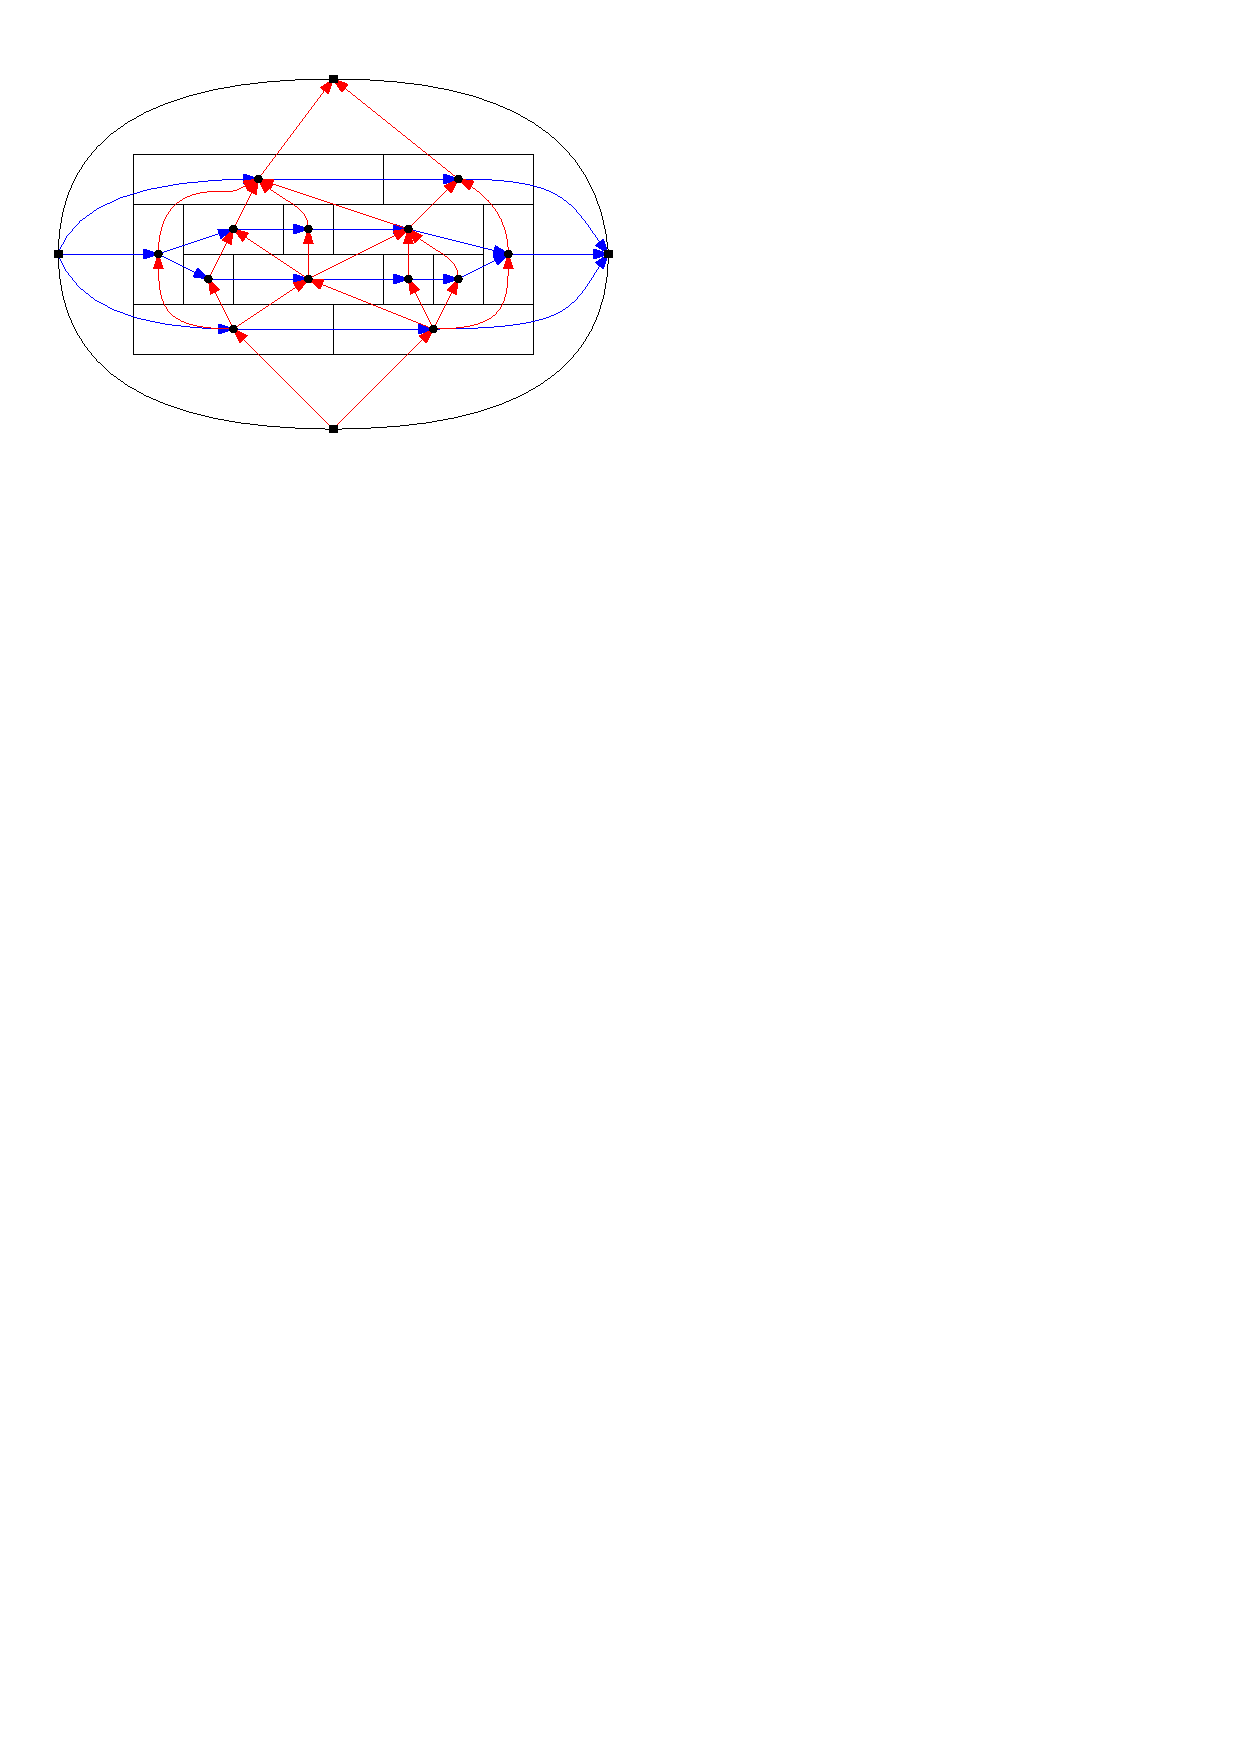
\includegraphics[scale=1]{rectangularDuals/img/relSegmentFaceRescale}
      \caption{}
      \label{fig:rect:relSegmentFace}
    \end{figure}

    Consider a face corresponding to a maximal segment.
    The number of interior vertices of both boundary paths without counting the split and merge vertices is the number of rectangles on the respective sides of the maximal segment.

    Hence a one-sided maximal segment corresponds to a face with one boundary path of length $2$\footnote{A boundary path can not have length $1$ since by construction of a \rel it encloses a maximal segment and thus has to go trough at least one intermediate rectangle/vertex.} and a $k$-sided maximal segment to face with shortest boundary path of length at most $k+1$.
